\documentclass[10pt,journal,compsoc]{IEEEtran}
\usepackage[spanish]{babel}
\usepackage{graphicx}
\usepackage{wrapfig}
\usepackage{listings}
\ifCLASSOPTIONcompsoc
  \usepackage[nocompress]{cite}
\else
  \usepackage{cite}
\fi

\ifCLASSINFOpdf
\else
\fi
\newcommand\MYhyperrefoptions{bookmarks=true,bookmarksnumbered=true,
pdfpagemode={UseOutlines},plainpages=false,pdfpagelabels=true,
colorlinks=true,linkcolor={black},citecolor={black},urlcolor={black},
pdftitle={Oz Mozart},
pdfsubject={Tarea Corta 4, Oz Mozart},
pdfauthor={Daniel, Wilbert, Anthony, Bryan},
}
\renewcommand{\lstlistingname}{Cuadro}
\lstset{
	extendedchars=true,
	frame = single, 
	language=Pascal, 
	framexleftmargin=3pt
}
\hyphenation{op-tical net-works semi-conduc-tor}

\begin{document}
\title{Oz Mozart}
\author{Daniel~Delgado,~\IEEEmembership{Estudiante,~ITCR,}
        Wilbert~Gonzales,~\IEEEmembership{Estudiante,~ITCR,}
        Anthony~Leandro,~\IEEEmembership{Estudiante,~ITCR,}
        and~Bryan~Mena,~\IEEEmembership{Estudiante,~ITCR}
}
\markboth{Lenguajes de Programaci\'on, Tarea Corta 4, Septiembre 2017}
{Shell \MakeLowercase{\textit{et al.}}: \LaTex}
\maketitle
\IEEEdisplaynontitleabstractindextext
\IEEEpeerreviewmaketitle

\section{Datos Historicos}
\begin{wrapfigure}{O}{0.3\textwidth}
	
\includegraphics[width=0.25\textwidth]{logo.png}
	\caption{\label{fig:Logo}Logo de Mozart}
\end{wrapfigure}

\par Concebido en 1991 por Gert Smolka en la universidad de Saarland y desarrollado en colaboraci\'on con Seif Haridi y Perter Van Roy en el SICS (Swedish Institute of Computer Science), desde 2005 recibe mantenimiento por \emph{Mozart Board}. Tiene herencia de:
\begin{itemize}
	\item Prolog
	\item Earlang
	\item LISP/Scheme
\end{itemize}
Oz es un lenguaje multiparadigma. Incluye las siguientes caracter\'isticas que lo hacen un lenguaje muy interesante para ense\~nar e investigar:\footnote{Datos tomados de \emph{Programming in Oz}, Ku\'snierczyk, W.}
\begin{itemize}
	\item Imperativo(Stateful) y funcional(Stateless)
	\item Data-Driven y Demand Driven programming
	\item Programaci\'on Relacional (L\'ogica) y Constraint-Propagation
	\item Concurrent and distributed programming
	\item Orientaci\'on a Objetos
\end{itemize}
\subsection{Mozart}
Mozart es un implementaci\'on de OZ, es un lenguaje de alto nivel desarrollado por la Universit\'e Catholique de Louvain para propositos educativos.

\section{Tipos de Datos\protect\footnote{Por comodidad, adjuntamos imagen con tipos de datos en el Ap\'endice A. Imagen tomada de \emph{Tutorial of Oz}}}
En Oz las variables no son variables, en OZ las variables son identificadores y no estan asignadas sino unificadas
\begin{itemize}
	\item Dynamically Type Language
	\item Cuando una variable es creada su tipo y su valor son desconocidos
	\item Solamente cuando una variables asociada con un valor se determina su tipo
\end{itemize}

\subsection{Estructuras B\'asicas de datos}
\begin{itemize}
	\item Numbers:
		\subitem Float: Es necesario que tengan decimales, en OZ 5.0 != 5
		\subitem Integer: OZ soporta formato binario, octal y hexadecimal para su representaci\'on
	\item Record: Compuesto de una etiqueta y un numero fijo de elementos
		\subitem Open Records: Igual que un Record pero con n\'umero variable de elementos 
		\subitem Agrupar datos
		\subitem Ejemplo de Record:
\begin{lstlisting}[language=Oz, caption = {Record}][linewidth=5.4cm]
<Etiqueta>(Feature:Field)
\end{lstlisting}
		Donde etiqueta es el nombre asociado al record, Feature es una etiqueta del elemento y field es el elemento, el conjunto de todas las etiquetas de Features se les llama arities (Algo similar a las keys en un diccionario de Python) 
		\subitem Se utiliza la notaci\'on "." para accesar a un elemento de un record. Ejemplo:
\begin{lstlisting}[language=Oz, caption = {Accesar al elemento de un Record}][linewidth=5.4cm]
{Browse <Etiqueta>.Feature}
\end{lstlisting}
		Donde etiqueta es el nombre del record y Feature la etiqueta del elemento que se quiere accesar
	\item Literals: Tipos donde sus miembros no tienen estructura interna
		\subitem *Atoms: Records vacios, solo que \'unicamente contine una etiqueta y no tiene ninguna caracter\'istica
		\subitem *Names: Es un identificador universal y \'unico, la unicamanera de crearlo es llamando a \verb|{NewName <Etiqueta>}|, su uso es importante ya que ayuda a la seguridad, como se ve en el arbol de tipos de datos un hijo de Name es Bool, esto hace que los valores true y false sean un Name por si solo, o sea \'unicos, universales e invariantes
	\item Tuplas
		\subitem Es un tipo de record, consiste de una etiqueta y valores
		\subitem Ejemplo
\begin{lstlisting}[language=Oz, caption = {Tupla}][linewidth=5.4cm]
<Etiqueta>(Feature:Field)
\end{lstlisting}
		\subitem En realidad las tuplas son records donde los features son numeros desde 1 hasta la cantidad de elementos de la tupla:
\begin{lstlisting}[language=Oz, caption = {Tupla}][linewidth=5.4cm]
<Etiqueta>(1:elemento1 2:elemento2)
\end{lstlisting}
	\item Listas: puede ser el atomo nil para representar una lista vacia o puede representar una tupla usando el operador infijo $\mid$ y dos argumentos, los cuales son la cabeza y la cola de la lista, otra representaci\'on utili es la lista cerrada representada por \verb|[ ]| y separando elementos por espacios. Tambien estan las listas representadas con los caracteres \verb|"| (doble comilla al inicio y al final) estos son los string, se puede utilizar el estatuto ForAll para iterar sobre cada elemento que posee
\end{itemize}
Algunas ideas sobre los tipos de datos anteriores:
\begin{itemize}
	\item \textbf{Chunks}
		\subitem Prmite al usuario introducir tipos de datos abstractos
	\item \textbf{Cell}
		\subitem Modificar el estado de la l\'ogica
	\item \textbf{Space}
		\subitem Resoluci\'on de problemas utilizando "\textit{Search Techniques}"
\end{itemize}

\section{Estructuras de Control y Expresiones}
\begin{figure}[h]
	\centering
	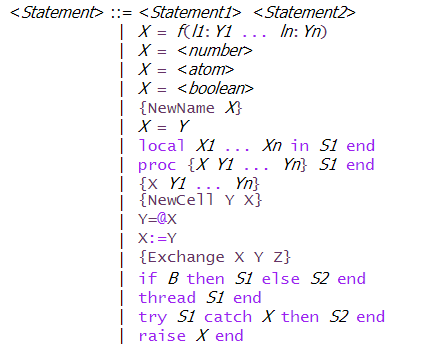
\includegraphics[width=0.5\textwidth]{struct.png}
	\caption{The Oz kernel language}
\end{figure}
\subsection{Operadores Condicionales}
\begin{tabular}{c p{3cm} p{5cm}}
	Operador & Significado\\
	\hline\hline\\
	$==$ & Igualdad\\
	$>$ & Mayor que\\
	$<$ & Menor que\\
	$>=$ & Mayor Igual que\\
	$<=$ &Menor Igual que\\
	\verb|\=| & Diferente\\
	\hline
\end{tabular}
\subsection{Operadores Booleanos}
\begin{tabular}{c p{3cm} p{5cm}}
	Operador & Significado\\
	\hline\hline\\
	$false$ & Valor de falsedad\\
	$true$ & Valor de Verdad\\
	$Not$ & Negaci\'on L\'ogica\\
	$Or~/~And$ & Or L\'ogico* And L\'ogico\\
	$orelse~/~andthen$ & Short circuit de los anteriores\\
	\hline
\end{tabular}
\subsection{Declaraci\'on de variables}
Para la declaraci\'on de variables que pertenecen a un scope dado se utiliza
\begin{lstlisting}[language=Oz, caption = {Variables en un scope}][linewidth=5.4cm]
local X Y Z in S end
\end{lstlisting}
El c\'odigo anterior crear 3 variables (X, Y, Z) y ejecuta S. Usualmente las variables inician con may\'uscula seguido de cualquier cantidad de caracteres alfa numericos. Otra manera de declarar variavles es:
\begin{lstlisting}[language=Oz, caption = {Variables en un scope}][linewidth=5.4cm]
declare X Y Z in S
\end{lstlisting}
Lo que esto hace es que X, Y, Z sean visibles globalmente en S y en los estatutos que sigan a S
\par En Oz hay pocas maneras de asociar variables a un valor, la usual es utilizar el operador infijo $"="$, ahora bien, si una variable ya contiene un valor la operaci\'on es considerada un test.

\subsubsection{¿Qu\'e pasa si se hace X = Y?}
Cuando se crea una variable se le asigna un espacio en memoria, un nodo, este nodo al inicio tiene valor y tipo desconocido, cuando las referencias a esa variable no existen se inicia un proceso de garbage collection para liberar los nodos que utilizaba esta varaible, cuando se utiliza la operaci\'on $"="$ intentar\'a unificar los valores de X y Y copiando sus nodos. La operaci\'on $"="$ se conoce como \emph{incremental tell} o \emph{unification}, algunos de sus resultados dependiendo del contexto:
\begin{itemize}
	\item Si las etiquetas X y Y pertenecen al mismo nodo la operaci\'on esta completa
	\item Si X no esta asociado se unifica el nodo de X con el nodo de Y, o sea todas las referencias a X pasan a ser referencias a Y
	\item Si X y Y contienen Records Rx y Ry respectivamente:
		\subitem Si los records Rx y Ry tienen diferentes etiquetas o arities se lanza un exception
		\subitem De otra manera los features de los records son unificados
\end{itemize}

\subsection{Operador de Igualdad}
Para probar una igualdad se utiliza l c\'odigo:
\begin{lstlisting}[language=Oz, caption = {Variables en un scope}][linewidth=5.4cm]
{Value.'==' X Y R}
\end{lstlisting}
Lo que se hace es probar si X es igual a Y y dejar el resultado en R. La operaci\'on:
\begin{itemize}
	\item Retorna true si los elementos tienen la misma estructura y los mismos valores o si son referencias al mismo nodo en memoria
	\item Retorna false si los elementos tienen estructuras o valores diferentes
	\item Se suspende cuando los nodos son diferentes pero existe un elemento sin asociar a un valor. Como Oz es un lenguaje concurrente cuando pasa esto el hilo que ejecut\'o el c\'odigo se suspende tambien.
\end{itemize}
Tambien se puede utilizar el operador \verb|"=="| como infijo tal que R = X == Y donde se prueba si X y Y son iguales y se deja el resultado en R

\subsection{Estatutos IF}
\begin{lstlisting}[language=Oz, caption = {Variables en un scope}][linewidth=5.4cm]
if B then S1 else S2 end
\end{lstlisting}
Lo que hace:
\begin{itemize}
	\item Si B es true S1 se ejecuta
	\item Si B es false S2 se ejecuta
	\item Si B no es un valor Booleano una exception ocurre
	\item Si B no tiene un valor asociado el hilo ejecutando se suspende 
\end{itemize}
Importante mencionar que la palabra reservada \emph{skip} funciona como el \emph{continue} en Python, adem\'as existe la abreviaci\'on \emph{elseif} que vendr\'ia siendo algo similar al \emph{elif} en Python:
\begin{lstlisting}[language=Oz, caption = {Variables en un scope}][linewidth=5.4cm]
if B1 then S1 elseif B2 then S2 else skip end
\end{lstlisting}

\subsection{Estatutos CASE}
\begin{lstlisting}[language=Oz, caption = {Variables en un scope}][linewidth=5.4cm]
case E 
of Pattern_1 then S1 
[] Pattern_2 then S2 
[] Pattern_3 then S3
[] ...
...
else S end
\end{lstlisting}
\subsubsection{Semantica}
Lo que hace el estatuto case es evaluar E con los $patrones_i$ esto de izquierda-derecha y \emph{depth-first}. Lo que hace:
\begin{itemize}
	\item Si E hace match con el $patron_i$ y E no esta siendo utilizado la instrucci\'on $S_i$ se ejecuta
	\item Si E hace match con el $patron_i$ pero E se esta utilizando se suspende el hilo
	\item Si E no hace match con el $patron_i$ se intenta con el $patron_i+1$ asi hasta alcanzar el else que se ejecutaria por defecto
	\item Dado sea el caso que la parte del \emph{else} sea omitida si E no hace match con algun $patron_i$ se lanza un exception
\end{itemize}

\subsection{Loops}
\subsubsection{For}
El procedimiento {For From To Step P} es una abstracci\'on de un for qu aplicac el prodecimiento P, From y To son integers que denotan el inicio y el fin del ciclo, Step es otra integer que indica el incremento (o decremento) en From para llegar a To. Un ejemplo de For:
\begin{lstlisting}[language=Oz, caption = {For}][linewidth=5.4cm]
{For 1 10 1 Browse}
\end{lstlisting}
El c\'odigo anterior mostrar\'a los n\'umeros de 1 al 10. Ejemplo m\'as general
\begin{lstlisting}[language=Oz, caption = {For}][linewidth=5.4cm]
local 
  proc {HelpPlus C To Step P}
    if C=<To then 
      {P C} {HelpPlus C+Step To Step P} 
    end 
  end 
  proc {HelpMinus C To Step P}
    if C>=To then 
      {P C} {HelpMinus C+Step To Step P} 
    end 
  end 
  in proc {For From To Step P}
    if Step>0 then 
      {HelpPlus From To Step P}
    else 
      {HelpMinus From To Step P} 
    end 
  end 
end
\end{lstlisting}

\subsection{Manejo de Excepciones}
Para lanzar una excepci\'on se utiliza
\begin{lstlisting}[language=Oz, caption = {Variables en un scope}][linewidth=5.4cm]
raise E end
\end{lstlisting}
donde E es una expresi\'on de error
Usualmente se utiliza un try-statement para manejar estos errores:
\begin{lstlisting}[language=Oz, caption = {Variables en un scope}][linewidth=5.4cm]
try S1 catch X then S2 end
\end{lstlisting}
La anterior es la forma m\'as simplificada de un try-statement:
\begin{lstlisting}[language=Oz, caption = {Variables en un scope}][linewidth=5.4cm]
try S catch 
Pattern_1 then S1 
[] Pattern_2 then S2 
... 
[] Pattern_n then Sn 
finally 
S_final 
end
\end{lstlisting}
Lo anterior se puede utilizar asemejando el try catch de Java con varios bloques catch y el bloque finally


\subsection{Procedimientos}
\begin{lstlisting}[language=Oz, caption = {Variables en un scope}][linewidth=5.4cm]
proc {P X1 ... Xn} S end
\end{lstlisting}
El c\'odigo anterior lo que hace es crear una lambda expression \'unica lo que lo hace diferente a todos los dem\'as procedimientos existentes, esa expresi\'on esta asociada con el valor P. Como dato curioso, la equicvalencia de procedimientos se realiza mediante su etiqueta o nombre. Ejemplo:
\begin{lstlisting}[language=Oz, caption = {Obtener el mayor entre dos n\'umeros}][linewidth=5.4cm]
local Max X Y Z in 
	proc {Max X Y Z}
		if X >= Y then Z = X 
		else Z = Y end 
	end 
	X = 5
	Y = 10
	{Max X Y Z} {Browse Z}
end
\end{lstlisting}

\subsection{Funciones}
\begin{lstlisting}[language=Oz, caption = {Variables en un scope}][linewidth=5.4cm]
fun {F X1 ... Xn} S E end
\end{lstlisting}
Como se puede apreciar la sintaxis de una funci\'on es muy similar a la de un procedimiento. Oz permite ciertas formas de optimizaci\'on tail-recursion 

\subsection{Funciones y procedimientos An\'onimos}
La idea detras de un procedimiento an\'onimo es que la funci\'on o procedimiento no esta asociada con una etiqueta generalmente son usada para procedimientos o funciones que no son longevas. En mozart se utiliza el simbolo \emph{\$} en vez de pasar la etiqueta que contendria la funcion un ejemplo de esto
\begin{lstlisting}[language=Oz, caption = {Variables en un scope}][linewidth=5.4cm]
fun {$ X1 ... Xn} ...end
\end{lstlisting}
La funci\'on anterior no estaria asociada con una etiqueta simplemente existe. Unejemplo \'util de esto:\footnote{Tomado de \emph{Tutorial of Oz}}
\begin{lstlisting}[language=Oz, caption = {Variables en un scope}][linewidth=5.4cm]
local 
  Max = proc {$ X Y Z}
          if X >= Y then Z = X
          else Z = Y end 
        end 
  X = 5
  Y = 10
  Z
in 
  {Max X Y Z} {Browse Z}
end
\end{lstlisting}

\section{M\'odulos e Interfaces}
Com\'unmente los modulos (o paquetes) son un grupo de procedimientos, valores, entre otros que se encuentran contenidos en un mismo lugar con el fin de brindar un conjunto de servicios relacionados, usualmente estos modulos contienen procedimientos privados que solo son accesibles dentro de si. En Oz se utiliza \emph{functor} para identificar miembros de un m\'odulo

\section{Orientaci\'on a Objetos}
En Oz una clase es un Chunk que contiene:
\begin{itemize}
	\item Una colecci\'on de m\'etodos
	\item Descripci\'on de los atributos que cada instancia tendr\'a
	\item Descripci\'on de los features que cada instancia de la clase tendr\'a (Un feature es una variable inmutable accesada por feature-name)
	\item Son simplemente descripciones de como un objeto se debe comportar
\end{itemize}
Ejemplo de una clase:
\begin{lstlisting}[language=Oz, caption = {Variables en un scope}][linewidth=5.4cm]
class Counter 
  attr val
  meth browse 
    {Browse @val}
  end 
  meth inc(Value)
    val := @val + Value
  end 
  meth init(Value)
    val := Value
  end 
end
\end{lstlisting}
Algunos datos importantes:
\begin{itemize}
	\item Para clases an\'onimas se utiliza el s\'imbolo  \emph{\$}
	\item  La llamada a un metodo toma como argumento impl\'icito el objeto actual (self)
	\item Existe una clase trivial (Base Object), el objetivo es que los hijos que la implementen no necesariamente tienen una funci\'on de inicializaci\'on
	\item es posible definir una clase abstracta donde los m\'etodos se dejan sin especificaci\'on
\end{itemize}

Para definir una clase se utiliza la palabra clave \emph{class}, para los atributos se definen con \emph{attr} para los features(similares a los records) se utiliza \emph{feat} y los m\'etodos con \emph{meth}; para herencia se utliza la palabra reservada \emph{from}, para accesar a un atributo se utiliza @<AttrName>, para llamar a un m\'etodo de una clase se utiliza <Class Name>, <Method Name>(..)

\subsection{\textquestiondown Para que se utiliza \emph{self}?}
Como en muchos lenguajes de Orientaci\'on a objetos, self se utiliza en vez de clases especificas, algo así como un binding din\'amico, donde \emph{self} toma\'a el valor de la clase desde la cual se invoca alg\'un elemento

\subsection{Atributos}
Como ya se dijo anteriormente, los atributos se declaran utilizando la palabra reservada \emph{attr}.
\begin{itemize}
	\item Los atributos son privados y solo los puede manipular el objetos que los contiene, la \'unica manera de modificar un atributo fuera de la clase es que la misma clase tenga m\'etodos para hacerlo
	\item Son \emph{Cells} que se pueden asignar, reasignar y accesar a voluntad
\end{itemize}

\subsection{Argumentos por Default para un M\'etodo}
\par Algunas veces en llamada a m\'etodos puede suceder que se desee no brindar un parametro, para esto existen los valores por default. Lo que se hace es asignar al argumento que no recibi\'o un valor un valor por default, esto se hace con el siguiente co\'odigo:
\begin{lstlisting}[language=Oz, caption = {Variables en un scope}][linewidth=5.4cm]
meth m(X Y d1:Z<=0 d2:W<=0) ... end
\end{lstlisting}
En caso que no se un valor para d1 o d2 se asume el valor de 0

\subsection{Herencia}
En Oz la herencia multiple esta implementada, se considera una clase (B) superclase de otra (A) si:
\begin{itemize}
	\item La clase B aparece despues de la declaraci\'on \emph{from} de la clase A
	\item La clase B es superclase de una clase C que aparece en la declaracion \emph{from} de la clase A
\end{itemize}
La herencia es una herramienta para construir clase apartir de clases ya existentes dandole un rango de metodos y atributos que tendr\'a la nueva clase. Un m\'etodo de la clase A sobre escribe cualquier m\'etodo con la misma etiqueta que posean sus superclases. No se permiten herencias ciclicas, esto es:
\begin{lstlisting}[language=Oz, caption = {Variables en un scope}][linewidth=5.4cm]
class A from B ... end 
class B from A ... end
\end{lstlisting}
No se permite que en herencia dos superclases (o m\'as) tengan m\'etodos atributos o features con el mismo tag esto no se evalua en tiempo de compilación sino en tiempo de ejecuci\'on cuando se crea una instancia del objeto y se intenta acceder al atributo o m\'etodo con el tag repetido 

\section{Caracter\'isticas}
\begin{itemize}
	\item Compilado o Interpretado, implementado en la plataforma Mozart
	\item Seguro, las entidades son creadas y pasadas explicitamente, esto significa que una aplicaci\'on no puede accesar o dar acceso a referencias que no se le han dado o creado en si misma
	\item Multiparadigma
		\subitem Orientaci\'on a Objetos
		\subitem Programaci\'on L\'ogica
		\subitem Programaci\'on Concurrente
			\subsubitem Threads Din\'amicos
\end{itemize}

\section{Ventajas}
\begin{itemize}
	\item Lenguaje Multiparadigma
	\item Concurrencia, hilos de pesos ultraligeros
	\item Lenguaje flexible
\end{itemize}

\section{Desventajas}
\begin{itemize}
	\item Debido a la flexibilidad es un poco lento, se han realizado pruebas donde OZ es 50\% m\'as lento que un compilador de C
\end{itemize}

\begin{thebibliography}{1}
	
	\bibitem{OzHomePage}
	Oz Mozart Home Page, http://mozart.github.io/
	
	\bibitem{MozartProgrammingSystem}
	\emph{Mozart Programming System}, P. Alarcon, H. Spakes, J. Ward; Arkansas Tech University
	
	\bibitem{TutorialOz}
	\emph{Tutorial of Oz}, S. Haridi, N. Franzén, Recuperado de:
	http://mozart.github.io/mozart-v1/doc-1.4.0/tutorial/index.html
	
	\bibitem{ReviewOfOz}
	\emph{A review of Oz and its implementation with Mozart}, Philippe Giabbanelli, Bishop’s University, Recuperado de: http://aqualonne.free.fr/Teaching/csc/oz.pdf
\end{thebibliography}

\appendices
\onecolumn
\section{}
\begin{figure}
	\centering
	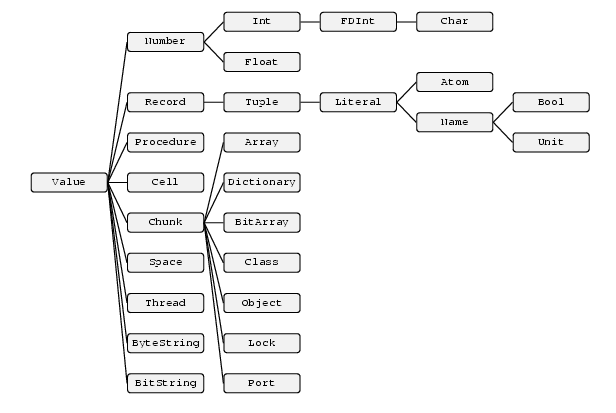
\includegraphics[width=\textwidth]{datos.png}
	\caption{\label{fig:Datos}Tipos de Datos, Tomado de \emph{Tutorial of Oz}}
\end{figure}

\end{document}


